\documentclass[11pt]{article}
\usepackage[margin=2.6cm]{geometry}
\usepackage{amsmath,amssymb,amsthm}
\usepackage{graphicx}
\usepackage{booktabs}
\usepackage{tikz}
\usepackage[colorlinks=true,linkcolor=blue,citecolor=blue]{hyperref}

\newcommand{\Li}{\mathrm{Li}}
\newcommand{\eps}{\epsilon}
\newcommand{\CT}{\mathrm{CT}}
\newcommand{\fin}{\mathrm{fin}}

\title{Two-loop pentabox with one lightlike leg:\\ nested local infrared subtraction and integrated counterterms}
\author{}
\date{}

\begin{document}
\maketitle

\noindent
This note constructs the complete nested local infrared subtraction for the planar two-loop pentabox
with a single lightlike external leg and four off-shell legs, following the protocol of
Ref.~\cite{AS}, and integrates every counterterm analytically through the pole level.
The example is designed so that the entire infrared structure is carried by exactly two nested
collinear surfaces, and so that the genuine two-loop-collinear counterterm is governed by the
four-propagator fixed-fraction double-collinear kernel of the accompanying kernel
note~\cite{kernel}. A structurally new feature relative to the examples of Ref.~\cite{AS} appears:
the two-loop-collinear counterterm itself requires an auxiliary-mass ultraviolet improvement of one
of its subloops. All algebraic identities and local scaling statements quoted below have been
verified symbolically with exact rational kinematics, and the analytic building blocks have been
verified numerically; a summary of the checks is given in section~\ref{sec:verif}.

\section{Kinematics, routing, and integral}
\label{sec:kin}

We consider the six-vertex pentabox topology of figure~\ref{fig:topo}: a pentagon subloop glued to
a box subloop across a shared rung. All five external momenta are incoming,
\begin{equation}
p_1+p_2+p_3+p_4+p_5=0,\qquad
p_1^2=0,\qquad p_i^2=m_i^2\neq 0,\quad i=2,3,4,5 .
\label{eq:extkin}
\end{equation}
The single lightlike momentum $p_1$ enters the pentagon at the corner adjacent to the upper
endpoint of the rung. This placement is the essential design choice of the example: it will put the
lightlike corner pair, the top box line and the rung simultaneously on shell in the two-loop
collinear limit, producing precisely the four-propagator structure of the kernel of
Ref.~\cite{kernel}.

The independent loop momenta are $\ell_2$ (pentagon) and $\ell_1$ (box). The eight internal lines
are massless, with denominators (all $+i0$)
\begin{equation}
\begin{aligned}
&A_1=\ell_2^2, \qquad
A_2=(\ell_2+p_1)^2,\qquad
A_3=(\ell_2+p_1+p_2)^2,\qquad
A_4=(\ell_2+p_1+p_2+p_3)^2,\\[2pt]
&A_5=\ell_1^2,\qquad
A_6=(\ell_1+p_5)^2,\qquad
A_7=(\ell_1+p_5+p_4)^2,\qquad
A_8=(\ell_1+\ell_2)^2 .
\end{aligned}
\label{eq:props}
\end{equation}
The scalar integral and its generalization with a numerator are
\begin{equation}
I[N]=\int\frac{d^d\ell_1}{i\pi^{d/2}}\frac{d^d\ell_2}{i\pi^{d/2}}\,
\frac{N(\ell_1,\ell_2)}{A_1A_2A_3A_4A_5A_6A_7A_8},
\qquad d=4-2\eps .
\label{eq:I}
\end{equation}

\begin{figure}[t]
\centering
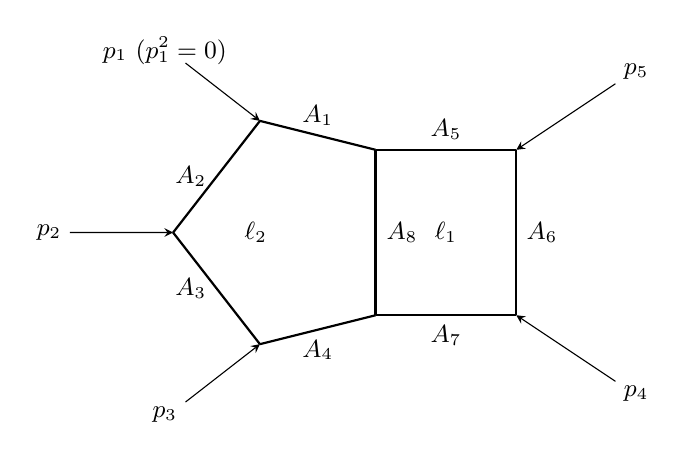
\begin{tikzpicture}[scale=1.05,>=stealth]
\coordinate (T) at (3,2);   \coordinate (B) at (3,0);
\coordinate (P1) at (1.6,2.35); \coordinate (P2) at (0.55,1); \coordinate (P3) at (1.6,-0.35);
\coordinate (R1) at (4.7,2);  \coordinate (R2) at (4.7,0);
\draw[thick] (T)--(P1) node[midway,above]{\small $A_1$};
\draw[thick] (P1)--(P2) node[midway,left]{\small $A_2$};
\draw[thick] (P2)--(P3) node[midway,left]{\small $A_3$};
\draw[thick] (P3)--(B) node[midway,below]{\small $A_4$};
\draw[thick] (T)--(R1) node[midway,above]{\small $A_5$};
\draw[thick] (R1)--(R2) node[midway,right]{\small $A_6$};
\draw[thick] (R2)--(B) node[midway,below]{\small $A_7$};
\draw[very thick] (T)--(B) node[midway,right]{\small $A_8$};
\draw[->] (0.7,3.05)--(P1); \node at (0.45,3.2) {\small $p_1$ ($p_1^2=0$)};
\draw[->] (-0.7,1)--(P2);   \node at (-0.95,1) {\small $p_2$};
\draw[->] (0.7,-1.05)--(P3);\node at (0.45,-1.2) {\small $p_3$};
\draw[->] (5.9,2.8)--(R1);  \node at (6.15,2.95) {\small $p_5$};
\draw[->] (5.9,-0.8)--(R2); \node at (6.15,-0.95) {\small $p_4$};
\node at (1.55,1) {\small $\ell_2$};
\node at (3.85,1) {\small $\ell_1$};
\end{tikzpicture}
\caption{Pentabox topology with all external momenta incoming. The pentagon carries $\ell_2$, the
box carries $\ell_1$, and the shared rung carries $\ell_1+\ell_2$. Only $p_1$ is lightlike.}
\label{fig:topo}
\end{figure}

Momentum conservation at the two rung endpoints closes if and only if $\sum_i p_i=0$, and it
implies $p_4+p_5=-(p_1+p_2+p_3)$. The hard structure of the diagram depends on exactly six
invariants,
\begin{equation}
m_2^2,\qquad
s_{12}=(p_1+p_2)^2,\qquad
m_{23}^2=(p_2+p_3)^2,\qquad
s_{123}=(p_1+p_2+p_3)^2,\qquad
m_5^2,\qquad
s_{15}=(p_1+p_5)^2 ,
\label{eq:invariants}
\end{equation}
together with the two derived identities, valid by momentum conservation and $p_1^2=0$,
\begin{equation}
(p_4+p_5)^2=s_{123},
\qquad
(p_1+p_4+p_5)^2=m_{23}^2 .
\label{eq:mcid}
\end{equation}
The masses $m_3^2$ and $m_4^2$ never appear in any collinear projection; $m_4^2$ enters only the
finite part of the single-collinear hard subgraph (section~\ref{sec:C12int}).

Throughout we use an auxiliary lightlike vector $\eta$,
\begin{equation}
\eta^2=0,\qquad p_1\cdot\eta=1,
\end{equation}
and the local longitudinal fractions
\begin{equation}
x(\ell_2)=(\ell_2+p_1)\cdot\eta,
\qquad
y(\ell_1)=\ell_1\cdot\eta .
\label{eq:fractions}
\end{equation}
The fraction $x$ is deliberately attached to the momentum $\ell_2+p_1$ of the line $A_2$ rather
than to $\ell_2$ itself: with
\begin{equation}
l=\ell_2+p_1,\qquad k=\ell_1,\qquad p=p_1,
\label{eq:kernelmap}
\end{equation}
the four jet propagators of section~\ref{sec:pinch} become \emph{verbatim} the propagator set
$\{\,l^2,\ (l-p)^2,\ k^2,\ (l+k-p)^2\,\}$ of the kernel note~\cite{kernel},
\begin{equation}
l^2=A_2,\qquad (l-p)^2=A_1,\qquad k^2=A_5,\qquad (l+k-p)^2=(\ell_1+\ell_2)^2=A_8,
\end{equation}
and the fractions \eqref{eq:fractions} coincide with the kernel variables $x=l\cdot\eta$,
$y=k\cdot\eta$.

\section{Infrared pinch surfaces}
\label{sec:pinch}

For a pinch surface $\rho$ the four-dimensional degree of divergence is
\begin{equation}
p_\rho=4L_S+2L_C-2N_S-N_C ,
\label{eq:degree}
\end{equation}
with $L_S$ ($L_C$) the number of independent soft (collinear) loop variables and $N_S$ ($N_C$) the
number of denominators of order $\delta^2$ ($\delta$). A surface is logarithmically divergent for
$p_\rho=0$.

\subsection{Jet lines and hard lines}
Since only $p_1$ is lightlike, every collinear surface is collinear to $p_1$. An internal line can
scale as $\delta$ on a $p_1$-collinear surface only if its momentum offset is $0$ or a multiple of
$p_1$; any line whose offset contains an off-shell external momentum is pinned hard. Reading off
\eqref{eq:props},
\begin{equation}
\underbrace{A_1,\ A_2,\ A_5,\ A_8}_{\text{jet lines}}
\qquad\qquad
\underbrace{A_3,\ A_4,\ A_6,\ A_7}_{\text{hard lines (carry }p_2,p_3,p_4,p_5)} .
\label{eq:jethard}
\end{equation}
The entire infrared structure therefore lives on four lines. In particular, the box subloop
participates in collinear physics only through its top corner line $A_5$ and the rung $A_8$.

\subsection{The two leading surfaces}

\paragraph{Genuine two-loop-collinear surface $C^{(2)}_{p_1}$.}
Defined by
\begin{equation}
\ell_2\to -(1-x)p_1,\qquad \ell_1\to y\,p_1,
\qquad 0<x<1,\quad 0<y<1-x ,
\label{eq:C2def}
\end{equation}
(the range of $y$ is the support of the rung fraction, cf.\ Ref.~\cite{kernel}).
Then $A_1,A_2,A_5,A_8\sim\delta$ while $A_3,A_4,A_6,A_7\sim 1$, so
\begin{equation}
L_C=2,\quad N_C=4,\qquad p_{C^{(2)}}=2\cdot2-4=0 .
\end{equation}
The surface is logarithmically divergent. Note the mechanism by which the box goes collinear: the
rung $A_8=(\ell_1+\ell_2)^2$ becomes a jet line only because \emph{both} loop momenta join the
$p_1$ jet.

\paragraph{Single-collinear surface $C_{12}$.}
Defined by
\begin{equation}
\ell_2\to -(1-x)p_1,\qquad 0<x<1,\qquad \ell_1 \text{ generic}.
\end{equation}
Then $A_1,A_2\sim\delta$ while $A_8\to(\ell_1-(1-x)p_1)^2$ stays hard for generic $\ell_1$, so
\begin{equation}
L_C=1,\quad N_C=2,\qquad p_{C_{12}}=2-2=0 ,
\end{equation}
again logarithmic. The surface $C^{(2)}_{p_1}$ is the $\ell_1$-collinear endpoint region contained
inside $C_{12}$; the two surfaces are nested.

\subsection{Absent surfaces}
\label{sec:absent}

\paragraph{No box single-collinear surface.} Taking $\ell_1\to y p_1$ with $\ell_2$ generic puts
only $A_5$ on shell: $A_6\to Q_6(y)$, $A_7\to Q_7(y)$ (see \eqref{eq:Qdefs}) are hard, and
$A_8\to(y p_1+\ell_2)^2$ is hard for generic $\ell_2$. A single vanishing denominator with
$L_C=1$ gives $p=2-1=1>0$; the configuration is not pinched at leading power. The box never
collinearizes on its own.

\paragraph{No two-collinear-pairs surface.} The graph contains a single collinear pair
($\{A_1,A_2\}$, at the unique lightlike corner). There is no second pair to combine with, hence no
product-of-pairs surface. The double-collinear region \eqref{eq:C2def} is \emph{not} an overlap of
two pairs; it is the endpoint of $C_{12}$ at which the box corner and the rung switch on.

\paragraph{No single-soft surfaces.} A soft line pinches the contour only if it is flanked by two
on-shell eikonal neighbours. Sending each line soft in isolation and counting on-shell
neighbours:
\begin{center}
\begin{tabular}{lll}
\toprule
soft line & forced configuration & eikonal neighbours\\
\midrule
$A_1$ & $\ell_2\to0$ & $A_2$ only\\
$A_2$ & $\ell_2\to-p_1$ & $A_1$ only\\
$A_3$ & $\ell_2\to-(p_1{+}p_2)$ & none\\
$A_4$ & $\ell_2\to p_4{+}p_5$ & none\\
$A_5$ & $\ell_1\to0$ & none\\
$A_6$ & $\ell_1\to-p_5$ & none (hard endpoint, $p_5^2\neq0$)\\
$A_7$ & $\ell_1\to p_1{+}p_2{+}p_3$ & none\\
$A_8$ & $\ell_1\to-\ell_2$ & none\\
\bottomrule
\end{tabular}
\end{center}
Every candidate has at most one eikonal neighbour, giving $N_C\le1$ and
$p\ge 4-2-1=1>0$. The only eikonal line in the whole graph is $A_1$ or $A_2$, sitting alone at the
single $p_1$ corner; the box attaches exclusively to off-shell legs and offers no eikonal partner.

\paragraph{No double-soft or soft-collinear surfaces.} The same one-corner eikonal capacity
suppresses all mixed configurations. Representative checks: both loops soft, $\ell_1,\ell_2\to0$,
gives $A_1,A_5,A_8\sim\delta^2$, only $A_2\sim\delta$, hence
$p=4\cdot2-2\cdot3-1=1>0$; $\ell_2$ soft with $\ell_1$ collinear gives $A_1\sim\delta^2$,
$A_2,A_5,A_8\sim\delta$, hence $p=4+2-2-3=1>0$, and identically for the mirror orientation. (The
soft-collinear surfaces of a fully massless topology are logarithmic because five lines can carry
$\{\ell_1,\ell_2,p_1\}$; here the off-shell legs reduce this to three, lifting the degree.)

\subsection{Leading-region table}

\begin{center}
\begin{tabular}{llll}
\toprule
pinch surface & defining configuration & on-shell lines & $p_\rho$\\
\midrule
$C^{(2)}_{p_1}$ & $\ell_2\to-(1-x)p_1$, $\ell_1\to y p_1$ & $A_1,A_2,A_5,A_8$ & $0$\\[2pt]
$C_{12}$ & $\ell_2\to-(1-x)p_1$, $\ell_1$ generic & $A_1,A_2$ & $0$\\
\bottomrule
\end{tabular}
\end{center}

\noindent
There are no soft, soft-collinear, box single-collinear, or two-pair surfaces. The complete
subtraction tower is $t_{2c}$ followed by $t_{12}$, ordered smallest region first.

\section{Counterterm construction}
\label{sec:CT}

\subsection{Frozen hard propagators}

On the two-loop-collinear surface \eqref{eq:C2def} each hard denominator freezes to a linear
interpolation in a single fraction. Using $p_1^2=0$ and \eqref{eq:mcid},
\begin{equation}
\begin{aligned}
A_3&=(\ell_2+p_1+p_2)^2\;\longrightarrow\;(x p_1+p_2)^2=m_2^2+2x\,p_1\!\cdot\! p_2
= m_2^2+x\,(s_{12}-m_2^2)\equiv Q_3(x),\\
A_4&\;\longrightarrow\;(x p_1+p_2+p_3)^2 = m_{23}^2+x\,(s_{123}-m_{23}^2)\equiv Q_4(x),\\
A_6&\;\longrightarrow\;(y p_1+p_5)^2 = m_5^2+y\,(s_{15}-m_5^2)\equiv Q_6(y),\\
A_7&\;\longrightarrow\;(y p_1+p_4+p_5)^2 = s_{123}+y\,(m_{23}^2-s_{123})\equiv Q_7(y) .
\end{aligned}
\label{eq:Qdefs}
\end{equation}
All four carry a $+i0$. It is convenient to name the slopes
\begin{equation}
q_3=s_{12}-m_2^2,\qquad
q_4=s_{123}-m_{23}^2,\qquad
q_6=s_{15}-m_5^2,\qquad
q_7=m_{23}^2-s_{123}=-q_4 ,
\label{eq:slopes}
\end{equation}
and to record the identity, which follows from \eqref{eq:slopes},
\begin{equation}
Q_7(y)=Q_4(1-y) .
\label{eq:Q7Q4}
\end{equation}
The frozen hard coefficient factorizes between the two fractions,
\begin{equation}
H_{2c}(x,y)=\frac{1}{Q_3(x)\,Q_4(x)\,Q_6(y)\,Q_7(y)}
= h_2(x)\,h_1(y),
\qquad
h_2=\frac{1}{Q_3Q_4},\quad h_1=\frac{1}{Q_6Q_7} .
\label{eq:H2c}
\end{equation}

\subsection{Two-loop-collinear layer: bare counterterm}

The approximation operator $t_{2c}$ keeps the jet product $A_1A_2A_5A_8$ exact and evaluates the
hard coefficient on the surface, using the local fractions \eqref{eq:fractions}:
\begin{equation}
t_{2c}F^{(0)}=\frac{H_{2c}\big(x(\ell_2),y(\ell_1)\big)}{A_1A_2A_5A_8},
\qquad
F^{(0)}=\frac{1}{A_1\cdots A_8}.
\end{equation}
The bare subtracted integrand can be written with a new numerator, in the pattern of
Ref.~\cite{AS},
\begin{equation}
(1-t_{2c})F^{(0)}=\frac{N^{(2c)}}{A_1\cdots A_8},
\qquad
N^{(2c)}=1-\frac{A_3A_4A_6A_7}{Q_3(x)\,Q_4(x)\,Q_6(y)\,Q_7(y)} .
\label{eq:N2c}
\end{equation}
In the collinear scaling ($\beta\sim\lambda^2$, $\ell_\perp\sim\lambda$, so $A_i\sim\delta=\lambda^2$
for jet lines) each hard propagator satisfies $A_i=Q_i+O(\lambda)$, the $O(\lambda)$ arising from
the $2p_j\!\cdot\!\ell_\perp$ terms. Hence every ratio in \eqref{eq:N2c} is $1+O(\lambda)$ and
\begin{equation}
N^{(2c)}\big|_{C^{(2)}_{p_1}}=O(\lambda)=O(\delta^{1/2}),
\end{equation}
lifting the logarithmic surface to power-suppressed (verified symbolically for two independent
approach directions). On the larger surface $C_{12}$, only $A_3,A_4$ freeze, so
\begin{equation}
N^{(2c)}\big|_{C_{12}}\longrightarrow 1-\frac{A_6A_7}{Q_6\big(y(\ell_1)\big)\,Q_7\big(y(\ell_1)\big)}
\neq0 :
\end{equation}
$C_{12}$ remains logarithmic and is removed by the next layer.

\subsection{Ultraviolet analysis of the bare counterterm and minimal improvement}
\label{sec:UV2c}

The bare counterterm has \emph{four} exact jet propagators, in contrast with five in the double-box
and triangle examples; this single missing power is what forces an ultraviolet improvement at this
layer. Since the hard coefficient depends only on the frozen fractions, it cannot damp regions in
which a loop momentum grows at fixed fraction. There are three such lightcone-UV regions. We count
degrees per dyadic shell: if $n$ scaling variables grow like $t$, the shell volume is $t^{\,n}$
per $d\ln t$, and convergence requires (integrand degree)$+n<0$.

\begin{itemize}
\item[(a)] \emph{$\ell_1$ transverse-UV at fixed $y$} ($\beta_1\sim\tau,\ \ell_{1\perp}^2\sim\tau$;
$n=2$). Only the two-propagator subloop $\{A_5,A_8\}$ is $\ell_1$-dependent; the integrand scales
as $\tau^{-2}$, total degree $-2+2=0$: \textbf{logarithmically divergent}. This is precisely the
$\Gamma(\eps)$ subloop pole of Eq.~(17) of Ref.~\cite{kernel}.
\item[(b)] \emph{$\ell_2$ transverse-UV at fixed $x$} ($n=2$). Here \emph{three} propagators are
$\ell_2$-dependent, $A_1,A_2$ \emph{and the rung} $A_8$: integrand $\sim t^{-3}$, total degree
$-3+2=-1$: \textbf{convergent}. The rung acts as a third damping propagator for the pentagon loop.
\item[(c)] \emph{Both transverse momenta large together at fixed fractions} ($n=4$: two $\beta$'s,
two $\tau$'s). All four jet propagators $\sim t$: integrand $t^{-4}$, total degree $-4+4=0$:
\textbf{logarithmically divergent} --- the same $\{A_5,A_8\}$ subloop divergence dragged along
while $\ell_2$ is also large.
\end{itemize}
All uniform (Euclidean) hard limits are convergent, since there $x,y=O(\Lambda)$ and
$H_{2c}\sim\Lambda^{-2}$ provides damping.

Both divergent regions are divergences of the $\{A_5,A_8\}$ pair alone. The minimal improvement is
therefore a single auxiliary-mass bracket on that pair,
\begin{equation}
\boxed{\;
t^{\mu}_{2c}F^{(0)}
=H_{2c}\big(x(\ell_2),y(\ell_1)\big)\,\frac{1}{A_1A_2}
\left[\frac{1}{A_5A_8}-\frac{1}{B_5B_8}\right],
\qquad B_i=A_i-\mu^2 .}
\label{eq:t2cmu}
\end{equation}
Pointwise, the bracket difference gains one power of the large scale
($\sim\mu^2(A_5+A_8)/(A_5A_8)^2$), turning the degrees in regions (a) and (c) into $-1$
(convergent), verified numerically (slopes $-2\to-3$ and $-4\to-5$). The subtraction of the
infrared surfaces is untouched: the cross term $H_{2c}/(A_1A_2B_5B_8)$ is $O(\lambda^4)$ at
$C^{(2)}_{p_1}$ (its would-be singular pair carries mass $\mu$), and at $C_{12}$ it is merely
log-singular, joining the inventory removed by $t_{12}$. The remainder after this layer is
\begin{equation}
F^{(2c)}=(1-t^\mu_{2c})F^{(0)}
=\frac{1}{A_1\cdots A_8}
-\frac{h_2\big(x(\ell_2)\big)\,h_1\big(y(\ell_1)\big)}{A_1A_2}
\left[\frac{1}{A_5A_8}-\frac{1}{B_5B_8}\right].
\label{eq:F2c}
\end{equation}

Two remarks place \eqref{eq:t2cmu} in context. First, the product-of-brackets structure for
\emph{disjoint} divergent subloops is the standard nested (BPHZ/$R$-operation) pattern, realized
with $\mu$-brackets exactly as in the overlap term of the regulated diagonal box, Eq.~(3.16) of
Ref.~\cite{AS}; there, however, the shared propagator is frozen and the two subloops decouple. Here
the rung stays exact and the loops remain coupled --- which is why the integrated counterterm is a
genuine two-loop kernel rather than a product of one-loop integrals. Second, only one subloop is
divergent in our case, so a single bracket suffices; the pentagon pair $\{A_1,A_2\}$ receives its
own bracket where power counting genuinely demands it, at the $C_{12}$ layer below. This mirrors
the asymmetry found in the two-loop triangle example, where only one of the two collinear pairs
required improvement.

\subsection{Single-collinear layer}
\label{sec:C12}

The final layer acts on the fully subtracted object,
\begin{equation}
F_{\fin}=(1-t^\mu_{12})\,F^{(2c)} .
\end{equation}
The operator $t_{12}$ keeps $A_1,A_2$ exact and evaluates the complementary factor at
$\ell_2=-(1-x)p_1$:
\begin{equation}
t_{12}F^{(2c)}=\frac{1}{A_1A_2}\,G^{(2c)}_{12}(x;\ell_1),
\qquad
G^{(2c)}_{12}(x;\ell_1)=\Big[A_1A_2\,F^{(2c)}\Big]_{\ell_2=-(1-x)p_1} .
\end{equation}
Both terms of \eqref{eq:F2c} contribute. Introducing the frozen rung
\begin{equation}
A_{8,12}(x;\ell_1)=\big(\ell_1-(1-x)p_1\big)^2 ,
\end{equation}
one finds
\begin{equation}
G^{(2c)}_{12}(x;\ell_1)
=\underbrace{\frac{h_2(x)}{A_5\,A_6\,A_7\,A_{8,12}}}_{\text{from }F^{(0)}}
\;-\;\underbrace{h_2(x)\,h_1\big(y(\ell_1)\big)
\left[\frac{1}{A_5A_{8,12}}-\frac{1}{B_5B_{8,12}}\right]}_{\text{from }-t^\mu_{2c}F^{(0)}} .
\label{eq:G12def}
\end{equation}
The first term is the genuine one-loop hard subgraph: a box in $\ell_1$ over
$\{A_5,A_6,A_7,A_{8,12}\}$ with an $x$-dependent lightlike external leg. The second term is the
nested two-loop-collinear subtraction at the same frozen $\ell_2$, carrying its $\mu$-bracket tail.
Near the collinear endpoint $\ell_1\to y p_1$ the first term approaches
$h_2 h_1(y)/(A_5A_{8,12})$, which cancels against the massless part of the second term; the
survivor $h_2h_1(y)/(B_5B_{8,12})$ is collinear-regular (mass $\mu$). Hence
$A_5A_{8,12}\,G^{(2c)}_{12}=O(\lambda)$ at the endpoint (verified symbolically):
$G^{(2c)}_{12}$ is pointwise integrable there, and it is ultraviolet convergent in $\ell_1$ (the
box by ordinary power counting; the bracket term by the same shell counting as region~(a) above,
now with degree $-3$ against $n=2$). Consequently the integrated hard function
\begin{equation}
G_{12}(x)=\int\frac{d^d\ell_1}{i\pi^{d/2}}\;G^{(2c)}_{12}(x;\ell_1)
\label{eq:G12int}
\end{equation}
is \emph{finite} as $\eps\to0$ --- its evaluation in section~\ref{sec:C12int} exhibits the pole
cancellation explicitly.

Finally, the pair $\{A_1,A_2\}$ is UV-improved with the same auxiliary mass (the bare $t_{12}$
carries the standard logarithmic $\ell_2$-UV divergence):
\begin{equation}
F_{\fin}=F^{(2c)}
-\left[\frac{1}{A_1A_2}-\frac{1}{B_1B_2}\right]G^{(2c)}_{12}\big(x(\ell_2);\ell_1\big) .
\label{eq:Ffin}
\end{equation}

\section{Analytic integration of the counterterms}
\label{sec:int}

With the sign conventions above, the counterterms added to the integrand are
$F^{\CT}_{2c}=-t^{\mu}_{2c}F^{(0)}$ and
$F^{\CT}_{12}=-\big[\tfrac{1}{A_1A_2}-\tfrac{1}{B_1B_2}\big]G^{(2c)}_{12}$, and
\begin{equation}
I[1]=I^{\CT}_{2c}+I^{\CT}_{12}+I_{\fin},
\qquad
I^{\CT}_{2c}=-\!\int t^{\mu}_{2c}F^{(0)},
\qquad
I^{\CT}_{12}=-\!\int \Big[\tfrac{1}{A_1A_2}-\tfrac{1}{B_1B_2}\Big]G^{(2c)}_{12},
\end{equation}
with $I_{\fin}$ finite in four dimensions.

\subsection{The two-loop-collinear kernel $K_4^{(0,\mu)}$}
\label{sec:K4}

Exposing the fractions with delta functions,
\begin{equation}
\int t^{\mu}_{2c}F^{(0)}
=\int_0^1\!dx\int_0^{1-x}\!dy\;H_{2c}(x,y)\,
\Big[K_4^{(0,0)}-K_4^{(0,\mu)}\Big](x,y;\eps),
\end{equation}
where $K_4^{(m_l,m_k)}$ is the fixed-fraction four-propagator double-collinear kernel of
Ref.~\cite{kernel} under the mapping \eqref{eq:kernelmap}: the $l$-pair $\{A_2,A_1\}$ carries mass
$m_l$ and the $k$-pair $\{A_5,A_8\}$ carries mass $m_k$, with $p^2=p_1^2=0$. In the notation of
Ref.~\cite{kernel},
\begin{equation}
X=1-x,\qquad
\lambda=\frac{y}{X},\qquad
\kappa=\lambda(1-\lambda),
\end{equation}
and the $k$-subloop result, Eq.~(17) of Ref.~\cite{kernel}, has scale
$C(l)=\mu_k^2(\lambda)-\kappa\,(p-l)^2$. For the massive corner $m_k=M_k=\mu$ one has
$\mu_k^2(\lambda)=\mu^2$, and for the massless $l$-pair with $p^2=0$ the residue representation,
Eq.~(29) of Ref.~\cite{kernel}, has
\begin{equation}
\Delta_0=0,
\qquad
A_1^{\rm note}=\mu^2,
\qquad
B_1=\frac{\kappa}{x} .
\end{equation}
The $t$-integral is then a pure Euler integral,
\begin{equation}
\int_0^\infty dt\;t^{-1-\eps}\big(\mu^2+B_1 t\big)^{-\eps}
=(\mu^2)^{-2\eps}\,B_1^{\eps}\;\frac{\Gamma(-\eps)\Gamma(2\eps)}{\Gamma(\eps)} ,
\end{equation}
(the standard formula $\int_0^\infty t^{a-1}(A+Bt)^{-c}dt=A^{a-c}B^{-a}\,B(a,c-a)$ continued to
$a=-\eps$, $c=\eps$; the two endpoint poles are the collinear $t\to0$ and transverse-UV
$t\to\infty$ singularities of the counterterm). Multiplying by the prefactor
$N_l(\eps)=\Gamma(\eps)/\big(X\,\Gamma(1-\eps)\big)$ of Ref.~\cite{kernel} and using
$\Gamma(-\eps)=-\Gamma(1-\eps)/\eps$, $\Gamma(2\eps)=\Gamma(1+2\eps)/(2\eps)$,
\begin{equation}
\boxed{\;
K_4^{(0,\mu)}(x,y;\eps)
=-\,\frac{\Gamma(1+2\eps)}{2\eps^{2}}\,
\frac{(\mu^{2})^{-2\eps}}{1-x}
\left[\frac{\lambda(1-\lambda)}{x}\right]^{\eps} .}
\label{eq:K4}
\end{equation}
No hypergeometric function survives at this mass corner; the leading behaviour
$-\tfrac{1}{2\eps^2(1-x)}$ matches the coefficient $c_{-2}=1/(2X)$ of Ref.~\cite{kernel} up to the
bracket sign. The massless corner $K_4^{(0,0)}$ has $A_1^{\rm note}=\Delta_0=0$ and is scaleless,
vanishing in dimensional regularization --- the usual cancellation of its infrared pole against
the spurious ultraviolet pole that the improvement is designed to control.

\subsection{Integrated two-loop-collinear counterterm}
\label{sec:I2c}

With $K_4^{(0,0)}=0$ the two minus signs compound, and substituting $y=\lambda(1-x)$,
\begin{equation}
I^{\CT}_{2c}
=+\int_0^1\!dx\int_0^{1-x}\!dy\;H_{2c}\,K_4^{(0,\mu)}
=-\frac{\Gamma(1+2\eps)}{2\eps^{2}}(\mu^{2})^{-2\eps}
\int_0^1\!dx\int_0^1\!d\lambda\;h_2(x)\,h_1\big(\lambda(1-x)\big)
\left[\frac{\lambda(1-\lambda)}{x}\right]^{\eps},
\end{equation}
(the Jacobian $X$ cancels the $1/X$ of the kernel). Organizing the $\eps$-expansion,
\begin{equation}
I^{\CT}_{2c}
=-\frac{\Gamma(1+2\eps)}{2\eps^{2}}(\mu^{2})^{-2\eps}
\Big[J_{0}+\eps J_{1}+\eps^{2}J_{2}+O(\eps^{3})\Big],
\qquad
J_n=\frac{1}{n!}\int_0^1\!\!dx\!\int_0^1\!\!d\lambda\;h_2\,h_1\,
\ln^{n}\!\frac{\lambda(1-\lambda)}{x} .
\label{eq:Jn}
\end{equation}
The integrands are regular on the closed square apart from integrable logarithmic endpoints; in
the Euclidean region defined below every quantity is real.

\subsection{Closed form of $J_0$}
\label{sec:J0}

The inner integral closes at weight one. Partial-fractioning
$h_1=\tfrac{1}{\Delta_{67}}\big[\tfrac{q_6}{Q_6}-\tfrac{q_7}{Q_7}\big]$ with
\begin{equation}
\Delta_{67}=q_6\,s_{123}-q_7\,m_5^2 ,
\label{eq:D67}
\end{equation}
(a constant: $q_6Q_7(y)-q_7Q_6(y)=\Delta_{67}$ identically), one finds
\begin{equation}
\frac{1}{X}\int_0^{X}dy\;h_1(y)
=\frac{\mathcal{L}(X)}{X\,\Delta_{67}},
\qquad
\mathcal{L}(X)=\ln\frac{Q_6(X)\,s_{123}}{Q_7(X)\,m_5^2} ,
\label{eq:Lambda}
\end{equation}
so that, after the change of variable $X=1-x$ and using $Q_4(1-X)=Q_7(X)$ from \eqref{eq:Q7Q4},
\begin{equation}
J_0=\frac{1}{\Delta_{67}}\int_0^1\frac{dX}{X\,\bar Q_3(X)\,Q_7(X)}
\Big[\ln\Big(1-\frac{X}{X_6}\Big)-\ln\Big(1-\frac{X}{X_7}\Big)\Big],
\qquad
\bar Q_3(X)\equiv Q_3(1-X)=s_{12}-q_3X .
\end{equation}
Both logarithms vanish at $X=0$, so the $1/X$ endpoint is integrable. The roots
\begin{equation}
X_3=\frac{s_{12}}{q_3},\qquad
X_7=\frac{s_{123}}{q_4},\qquad
X_6=-\frac{m_5^2}{q_6},
\qquad\text{with}\qquad
\frac{1}{X_3}=1-\frac{m_2^2}{s_{12}},\quad
\frac{1}{X_7}=1-\frac{m_{23}^2}{s_{123}},\quad
\frac{1}{X_6}=1-\frac{s_{15}}{m_5^2},
\label{eq:roots}
\end{equation}
all lie outside $[0,1]$ in the Euclidean region. Partial-fractioning
$\big[X\bar Q_3Q_7\big]^{-1}=\tfrac{1}{q_3q_4}\big[X(X-X_3)(X-X_7)\big]^{-1}$ by residues and
using the master integrals
\begin{align}
M_1(w)&=\int_0^1\frac{dX}{X}\,\ln\Big(1-\frac Xw\Big)=-\Li_2\Big(\frac1w\Big),\\
M_2(z,w)&=\int_0^1\frac{dX}{X-z}\,\ln\Big(1-\frac Xw\Big)
=\Li_2\Big(\frac{w-1}{w-z}\Big)-\Li_2\Big(\frac{w}{w-z}\Big)
+\ln\Big(\frac{w-1}{w}\Big)\ln\Big(\frac{1-z}{w-z}\Big),
\label{eq:M2}\\
M_2(w,w)&=\tfrac12\ln^2\Big(1-\frac1w\Big),
\end{align}
one obtains
\begin{equation}
\boxed{\;
J_0=\frac{1}{\Delta_{67}}\left\{
\frac{\Li_2(1/X_7)-\Li_2(1/X_6)}{s_{12}\,s_{123}}
+c_3\Big[M_2(X_3,X_6)-M_2(X_3,X_7)\Big]
+c_7\Big[M_2(X_7,X_6)-\tfrac12\ln^2\big(1-\tfrac1{X_7}\big)\Big]
\right\}\;}
\label{eq:J0}
\end{equation}
with the residue coefficients
\begin{equation}
c_3=\frac{1}{q_3q_4\,X_3(X_3-X_7)},
\qquad
c_7=\frac{1}{q_3q_4\,X_7(X_7-X_3)} .
\end{equation}
The master \eqref{eq:M2} is derived by one integration by parts against
$d\ln\!\big((X-z)/(-z)\big)$ followed by the substitution $t=(X-z)/(w-z)$; it was verified to 18
digits at six $(z,w)$ configurations, and \eqref{eq:J0} was verified against direct
two-dimensional integration to 18 digits.

$J_1$ and $J_2$ are weight-3 and weight-4 two-fold convolutions over the same alphabet
$\{x,\,1-x,\,\lambda,\,1-\lambda,\,X_3,\,X_6,\,X_7\}$; both are now in closed GPL form, obtained
with the fibration pipeline of section~\ref{sec:methods} (ancillary scripts
\texttt{pentabox\_finite.wl}, \texttt{pentabox\_pass3.wl}) and verified to $22$ digits at the two
Euclidean reference points; numerical reference values are given in section~\ref{sec:assembly}.

\subsection{Integrated single-collinear counterterm}
\label{sec:C12int}

With equal masses on the improved pair, the transverse integration of the bracket
$\big[\tfrac{1}{A_1A_2}-\tfrac{1}{B_1B_2}\big]$ at fixed fraction gives $0$ (scaleless) minus the
massive kernel $\tfrac{\Gamma(1+\eps)}{\eps}(\mu^2)^{-\eps}$ [Eq.~(3.20) of Ref.~\cite{AS} at
$m=M=\mu$], so the two minus signs again compound:
\begin{equation}
I^{\CT}_{12}
=+\,\frac{\Gamma(1+\eps)}{\eps}\,(\mu^{2})^{-\eps}
\int_0^1 dx\;G_{12}(x) .
\label{eq:ICT12}
\end{equation}
It remains to evaluate the two pieces of \eqref{eq:G12def}--\eqref{eq:G12int}.

\paragraph{Nested bracket term.}
The $\ell_1$-integral of the bracket piece is again the $k$-subloop of Ref.~\cite{kernel}: the
massless part is scaleless, and the massive part is Eq.~(17) of Ref.~\cite{kernel} with external
lightlike momentum $Xp_1$ and $C=\mu^2$, i.e.\
$\Gamma(\eps)(\mu^2)^{-\eps}/X$ on the support $0<y<X$. Using \eqref{eq:Lambda},
\begin{equation}
-\int\frac{d^d\ell_1}{i\pi^{d/2}}\;
h_2\,h_1\big(y(\ell_1)\big)\left[\frac{1}{A_5A_{8,12}}-\frac{1}{B_5B_{8,12}}\right]
=+\,h_2(x)\,\frac{\Gamma(1+\eps)}{\eps}(\mu^{2})^{-\eps}\,
\frac{\mathcal{L}(X)}{X\,\Delta_{67}} .
\label{eq:bracketterm}
\end{equation}

\paragraph{Box term.}
The subgraph $\{A_5,A_6,A_7,A_{8,12}\}$ is a one-loop box with massless internal lines. Reading
the incoming external legs from the propagator offsets $(0,\,p_5,\,p_5+p_4,\,-Xp_1)$, the cyclic
legs are
\begin{equation}
q_d=Xp_1,\qquad q_a=p_5,\qquad q_b=p_4,\qquad q_c=-(Xp_1+p_4+p_5),
\end{equation}
with virtualities and Mandelstam invariants (using \eqref{eq:mcid}; all verified symbolically)
\begin{equation}
q_d^2=0,\qquad q_a^2=m_5^2,\qquad q_b^2=m_4^2,\qquad
q_c^2=s_{123}+X(m_{23}^2-s_{123})=Q_7(X)=Q_4(x),
\end{equation}
\begin{equation}
s_B=(q_d+q_a)^2=Q_6(X),
\qquad
t_B=(q_a+q_b)^2=(p_4+p_5)^2=s_{123} .
\end{equation}
Thus the hard subgraph is the \emph{three-mass box} with one lightlike leg: exactly Box~5 of
Ref.~\cite{EZ}, $I_4^{D}(0,p_2^2,p_3^2,p_4^2;s_{12},s_{23})$ with massless internal lines, under
the dictionary
\begin{equation}
p_2^2\to m_5^2,\qquad p_3^2\to m_4^2,\qquad p_4^2\to Q_7(X),\qquad
s_{12}\to Q_6(X),\qquad s_{23}\to s_{123} ,
\label{eq:EZmap}
\end{equation}
and, accounting for the normalization of Ref.~\cite{EZ}
($I_4^{\rm EZ}=\mu^{2\eps}r_\Gamma^{-1}\int d^d\ell/(i\pi^{d/2})\cdots$ with
$r_\Gamma=\Gamma(1+\eps)\Gamma^2(1-\eps)/\Gamma(1-2\eps)$),
\begin{equation}
B_{3m}(x)=\int\frac{d^d\ell_1}{i\pi^{d/2}}\frac{1}{A_5A_6A_7A_{8,12}}
=r_\Gamma\,\big[I_4^{\rm EZ,\,Box\,5}\big]_{\mu=1} .
\end{equation}
Two structural facts make the assembly work.

First, the characteristic denominator of Box~5 obeys the exact identity (immediate from
$Q_6(X)=m_5^2+q_6X$, $Q_7(X)=s_{123}+q_7X$ and \eqref{eq:D67})
\begin{equation}
s_Bt_B-p_2^2\,p_4^2\;=\;Q_6(X)\,s_{123}-m_5^2\,Q_7(X)\;=\;X\,\Delta_{67} .
\label{eq:XD}
\end{equation}
Second, the singular part of Box~5,
\begin{equation}
\frac{r_\Gamma}{X\Delta_{67}}\cdot\frac{1}{\eps^{2}}
\Big[2\big((-s_B)^{-\eps}+(-t_B)^{-\eps}-(-m_5^2)^{-\eps}-(-m_4^2)^{-\eps}-(-Q_7)^{-\eps}\big)
+\tfrac{(-m_5^2)^{-\eps}(-m_4^2)^{-\eps}}{(-t_B)^{-\eps}}
+\tfrac{(-m_4^2)^{-\eps}(-Q_7)^{-\eps}}{(-s_B)^{-\eps}}\Big],
\label{eq:poleblock}
\end{equation}
has vanishing $1/\eps^2$ coefficient ($2-2=0$), and its single pole collapses, with the middle
mass $m_4^2$ dropping out, to
\begin{equation}
B_{3m}(x)\Big|_{\rm pole}
=-\,\frac{1}{\eps}\,\frac{\mathcal{L}(X)}{X\,\Delta_{67}}
=-\,\frac{1}{\eps}\,\frac{1}{X}\int_0^X dy\,h_1(y) ,
\end{equation}
which is \emph{exactly minus} the pole of the bracket term \eqref{eq:bracketterm}, including the
$\gamma_E$ terms ($r_\Gamma$ and $\Gamma(1+\eps)$ are both $1-\gamma_E\eps+O(\eps^2)$). This
cancellation is forced: $G^{(2c)}_{12}$ was shown to be pointwise integrable and UV convergent in
section~\ref{sec:C12}, hence finite; the collinear pole of the inner box must be removed by the
nested subtraction, and it is. The finite limit is
\begin{equation}
G_{12}(x)=h_2(x)\Big[\hat b(x)-\frac{\mathcal{L}(X)}{X\Delta_{67}}\,\ln\mu^{2}\Big]+O(\eps),
\label{eq:G12fin}
\end{equation}
with the $\mu$- and $\gamma_E$-free content, obtained from the $\eps^0$ term of
$r_\Gamma\times$\eqref{eq:poleblock} plus the finite dilogarithms of Box~5 of Ref.~\cite{EZ},
\begin{equation}
\begin{aligned}
\hat b(x)=\frac{1}{X\Delta_{67}}\Big[&
\ln^{2}(-s_B)+\ln^{2}(-t_B)-\ln^{2}(-m_5^2)-\ln^{2}(-m_4^2)-\ln^{2}(-Q_7)\\
&+\tfrac12\big(\ln(-m_5^2)+\ln(-m_4^2)-\ln(-t_B)\big)^{2}
+\tfrac12\big(\ln(-m_4^2)+\ln(-Q_7)-\ln(-s_B)\big)^{2}\\
&-2\,\Li_2\Big(1-\tfrac{m_5^2}{s_B}\Big)
-2\,\Li_2\Big(1-\tfrac{Q_7}{t_B}\Big)
+2\,\Li_2\Big(1-\tfrac{m_5^2\,Q_7}{s_B\,t_B}\Big)
-\ln^{2}\Big(\tfrac{s_B}{t_B}\Big)\Big],
\end{aligned}
\label{eq:bhat}
\end{equation}
where throughout $s_B=Q_6(X)$, $t_B=s_{123}$, $Q_7=Q_7(X)=Q_4(x)$, $X=1-x$. The mapped Box~5
expression, i.e.\ the combination \eqref{eq:poleblock}$+$dilogarithms, was verified at a Euclidean
point against an independent direct Feynman-parameter integration of the box (analytic integration
of one simplex direction, adaptive quadrature of the remaining two, four values of $\eps<0$, cubic
extrapolation to $\eps=0$), agreeing to $2\times10^{-4}$ relative --- sufficient to confirm every
dilogarithm coefficient.

Defining
\begin{equation}
\hat g_0=\int_0^1 dx\;h_2(x)\,\hat b(x),
\qquad\text{so that}\qquad
\int_0^1dx\,G_{12}\Big|_{\eps^0}=\hat g_0-J_0\ln\mu^{2}
\end{equation}
(the coefficient of $\ln\mu^2$ is $-\int h_2\,\mathcal{L}/(X\Delta_{67})=-J_0$ by
\eqref{eq:Lambda}), the single-collinear counterterm contributes
\begin{equation}
I^{\CT}_{12}
=\frac{\Gamma(1+\eps)}{\eps}(\mu^{2})^{-\eps}
\Big[\hat g_0-J_0\ln\mu^{2}+\eps\,g_1+O(\eps^{2})\Big] .
\label{eq:ICT12exp}
\end{equation}
The $O(\eps)$ coefficient $g_1$ requires the $O(\eps)$ term of the three-mass box, which is not
provided by Ref.~\cite{EZ}; it is needed only for the finite ($\eps^0$) assembly, not for the
poles. It is obtained in section~\ref{sec:methods} from the all-order one-fold
${}_2F_1$ representation of Ref.~\cite{DN} (Eq.~(22) there): the $\eps$-expansion of the
integrand yields $\hat b_1(x)$ --- the $O(\eps)$ box coefficient --- in closed weight-3 GPL form,
and $\beta_1=\int_0^1 dx\,h_2(x)\,\hat b_1(x)$ as a one-fold representation with $22$-digit
values at both Euclidean reference points; the remaining open item is only the closed weight-4
$x$-integral of $\hat b_1$, whose alphabet contains the two quadratic box roots.

\subsection{Assembled singularity structure}
\label{sec:assembly}

Collecting \eqref{eq:Jn} and \eqref{eq:ICT12exp},
\begin{equation}
I^{\CT}=I^{\CT}_{2c}+I^{\CT}_{12}
=-\frac{\Gamma(1+2\eps)}{2\eps^{2}}(\mu^{2})^{-2\eps}
\big[J_{0}+\eps J_{1}+\eps^{2}J_{2}\big]
+\frac{\Gamma(1+\eps)}{\eps}(\mu^{2})^{-\eps}
\big[\hat g_0-J_0\ln\mu^2+\eps g_{1}\big]+O(\eps) .
\end{equation}
Expanding, the $\ln\mu^2$ terms cancel between the two layers in both pole coefficients --- a
nontrivial consistency check: the artificial mass cannot contaminate the genuine infrared poles of
the pentabox. The result is
\begin{equation}
\boxed{\;
I^{\CT}
=-\frac{J_{0}}{2\eps^{2}}
+\frac{1}{\eps}\Big[\gamma_E\,J_{0}-\frac{J_{1}}{2}+\hat g_{0}\Big]
+O(\eps^{0}) ,\;}
\label{eq:poles}
\end{equation}
and, since $I[1]=I^{\CT}+I_{\fin}$ with $I_{\fin}$ finite, \eqref{eq:poles} \emph{is} the
predicted pole structure of the pentabox: a double pole from the nesting
$C^{(2)}_{p_1}\subset C_{12}$ (one logarithm per layer), with a coefficient $-J_0/2$ that is
already a weight-2 function of the six invariants \eqref{eq:invariants}, and a single pole of
weight $\le3$. The residual $\gamma_E$ reflects the mismatch of the natural $\Gamma$-normalizations
of the two layers and would be absorbed by an $e^{-\gamma_E\eps}$-type convention.

\paragraph{Reference values.}
At the Euclidean point
\begin{equation}
(m_2^2,\,m_4^2,\,m_5^2,\,s_{12},\,s_{123},\,m_{23}^2,\,s_{15})
=(-5,\,-3,\,-24,\,-7,\,-13,\,-14,\,-26),
\label{eq:euclpoint}
\end{equation}
where every $Q_i$ is strictly negative on $[0,1]$ and all roots \eqref{eq:roots} are real and
outside $[0,1]$ ($X_3=3.5$, $X_7=-13$, $X_6=-12$, $\Delta_{67}=2$), so that all quantities are
real:
\begin{equation}
\begin{aligned}
J_0&=\phantom{-}3.829615095208904272551\times10^{-5},\\
J_1&=-3.645278651337797191406\times10^{-5},\\
J_2&=\phantom{-}5.109747509667592746057\times10^{-5},\\
\hat g_0&=\phantom{-}1.793890330475915652717\times10^{-4},
\end{aligned}
\qquad
\begin{aligned}
c_{-2}&=-\tfrac{J_0}{2}=-1.914807547604452136\times10^{-5},\\[2pt]
c_{-1}&=\gamma_EJ_0-\tfrac{J_1}{2}+\hat g_0\\
&=\phantom{-}2.197205645392600987\times10^{-4} .
\end{aligned}
\label{eq:refvals}
\end{equation}
$J_0$ from \eqref{eq:J0} agrees with direct integration to 18 digits. For physical kinematics all
formulas continue with $s\to s+i0$ in every $(-s)^{-\eps}$, logarithm, and dilogarithm argument.

\section{Results}
\label{sec:results}

The complete singular structure of the pentabox is given by \eqref{eq:poles},
\begin{equation}
I^{\CT}
=-\frac{J_{0}}{2\eps^{2}}
+\frac{1}{\eps}\Big[\gamma_E\,J_{0}-\frac{J_{1}}{2}+\hat g_{0}\Big]
+O(\eps^{0}),
\end{equation}
with $J_0$ (weight 2, Eq.~\eqref{eq:J0}), $J_1$ and $\hat g_0$ (weight 3) and $J_2$ (weight 4)
all in closed GPL form over the alphabet $\{x,1-x,X_3,X_6,X_7\}$ and its $\lambda$-images
(section~\ref{sec:methods}; machine-readable forms in the ancillary files). All $\mu$-dependence
of the counterterm enters through the two overall exponentials
$I^{\CT}=(\mu^2)^{-2\eps}A(\eps)+(\mu^2)^{-\eps}B(\eps)$, and the finite part splits as
\begin{equation}
\boxed{\;
I^{\CT}\big|_{\eps^0}=A_{\rm fin}+\big(J_1-\hat g_0\big)\ln\mu^2+\tfrac{J_0}{2}\ln^2\mu^2,\;}
\qquad
A_{\rm fin}=\beta_1-\tfrac{J_2}{2}+\gamma_E\big(J_1-\hat g_0\big)
-\tfrac{\gamma_E^2}{2}J_0-\tfrac{\pi^2}{12}J_0,
\label{eq:finres}
\end{equation}
with $\beta_1=\int_0^1dx\,h_2\,\hat b_1$ now also in \emph{closed} weight-4 GPL form
(section~\ref{sec:methods}), so that $A_{\rm fin}$ is fully explicit. At the reference point
\eqref{eq:euclpoint},
\begin{equation}
J_2=5.109747509667592746057\times10^{-5},\qquad
\beta_1=4.670736153857860632218\times10^{-5},\qquad
A_{\rm fin}=-1.413056930983497823\times10^{-4},
\end{equation}
complementing \eqref{eq:refvals}; every closed form reproduces its defining integral to at
least $20$--$22$ digits at three independent Euclidean points.

\section{Computational methods}
\label{sec:methods}

\paragraph{Fibration at weight $\le2$ and the constant-fitting wall.}
The reduction of the convolutions to GPLs in the fraction $x$ requires rotating
$G$-functions with $x$-dependent letters into a fibration basis $G(\vec a;x)$ with constant
letters. The library routine (\texttt{ToFibrationBasis}, PolyLogTools~1.4) aborts for this
kinematics: its constant-fitting step insists on reducing the $x=0$ boundary constants to
multiple zeta values, whereas here they are generic-argument polylogarithms
($\mathrm{Li}_2$ at the rational roots $1/X_3,1/X_6,1/X_7$ and their images). The bypass used
throughout is symbol-level fibration, $\texttt{FiberSymbol}[\texttt{SymbolMap}[\,\cdot\,],\{x\}]$,
which matches the symbol only and therefore never touches the boundary constants; the
beyond-symbol constant is then fixed \emph{in closed form} at the base point $x=0$, where every
GPL collapses to explicit polylogarithms at the rational roots (never MZV-reduced). This closes
all weight-$\le2$ fibrations and was validated by reproducing $J_0$ of \eqref{eq:J0} to $22$
digits through the full pipeline.

\paragraph{Weight $\ge3$: derivative--primitive construction.}
At weight $3$ the fibration deficit involves undetermined \emph{weight-2} boundary constants
whose individual symbol tensors $a\otimes b$ are not integrable, so they cannot be resolved
one by one. They are avoided entirely by the derivative--primitive construction: for a
weight-3 object $g(x)$ with $x$-dependent letters,
$g(x)=g(0)+\int_0^x dt\,\partial_t g(t)$, where $\partial_t g$ is weight~2 (total-differential
formula, only $d\ln$ coefficients with simple poles), is fibrated by the weight-$\le2$ method,
and the primitive is the $M_3$-type master
$\int_0^x dt\,G(\vec w;t)/(t-z)=G(z,\vec w;x)$, extended to higher-order poles by integration
by parts. No numerical fitting (PSLQ or otherwise) enters at any stage. This closes the
weight-4 convolution $J_2$ (verified to $22$ digits at both Euclidean reference points), with
$J_0$, $J_1$, $\hat g_0$ passing unchanged as regression guards.

\paragraph{The three-mass box at $O(\eps)$.}
The single-collinear finite part requires the $O(\eps)$ term of the three-mass box. Starting
from the all-order one-fold representation of Ref.~\cite{DN}, Eq.~(22), the integrand is
expanded with
${}_2F_1(1-\eps,\eps;1+\eps;w)=1-\eps L-\eps^{2}\big(2\,\mathrm{Li}_2(w)+\tfrac12L^{2}\big)
+O(\eps^{3})$, $L=\ln(1-w)$: the $\eps^{0}$ term reproduces $\hat b(x)$ of \eqref{eq:bhat} and
the pole reproduces $-\mathcal L(X)/(X\Delta_{67})$ to $32$ digits (fixing the normalization
$B_{3m}=2\,\bar I_{3m}$). The $O(\eps)$ $z$-integral is performed with the same partial-fraction
masters plus the dilogarithm master
$\int_0^1 dz\,\mathrm{Li}_2(w(z))/(z-r)
=\tfrac{\pi^2}{6}\ln\!\big(1-\tfrac1r\big)+\int_0^1 dz\,\ln\!\big(\tfrac{z-r}{-r}\big)
\ln(1-w)\,d\ln w$, giving $\hat b_1(x)$ in closed weight-3 GPL form whose alphabet contains, in
addition to the rational roots, the two quadratic roots of $A_i(z)-z(1-z)\,(-m_4^2)$
(the box Landau letters). The closed form was verified to $36$ digits against direct
integration; at the second Euclidean point the letter $z_D$ lies inside $(0,1)$ and the GPL
combination continues correctly across it (imaginary parts cancel; checked against a
contour-deformed direct integral).

\paragraph{The weight-4 integral $\beta_1$.}
The alphabet of $\hat b_1(x)$ contains a single $x$-dependent radicand, the quadratic
$d_1(x)$ with perfect-square leading coefficient $(q_6-q_7)^2$ (all other radicands are
$x$-independent constants), so $\beta_1=\int_0^1dx\,h_2\hat b_1$ is Euler-rationalizable in
principle. In practice the rationalizing map inflates the remaining letters; the closed form is
obtained instead by \emph{exchanging the integration order}: at fixed $z$ the $\eps$-expanded
integrand of the box representation is rational-\emph{linear} in $x$, so the inner $x$-integral
closes over letters \emph{rational} in $z$. The outer $z$-integral is then fibrated with the same
derivative--primitive construction, extended by (i) exact conversion of the boundary logarithms
and dilogarithms with $z$-adic order extraction at the base point, and (ii) a registry of
irreducible quadratic denominators whose roots are carried as symbolic radicals (three constant
discriminants), residues being evaluated modulo the source quadratic. The $x$-dependent radical
never enters the integration variable --- all square roots are confined to \emph{constant}
letters --- and $\beta_1$ closes as a weight-4 GPL combination, reproducing its defining integral
to $22$ digits at the two reference points and to $20$ digits at a third point at which all three
discriminants change sign (a full branch-configuration flip). No numerical fitting (PSLQ or
otherwise) enters at any stage.

\section{Summary of verifications}
\label{sec:verif}

All symbolic checks were performed with exact rational external momenta
($p_1=(1,0,0,1)$ lightlike, $\eta=\tfrac12(1,0,0,-1)$, generic off-shell $p_2,\dots,p_5$), for at
least two independent approach directions per surface; numerical checks in 30-digit arithmetic.

\begin{center}
\small
\begin{tabular}{ll}
\toprule
check & result\\
\midrule
momentum-conservation identities \eqref{eq:mcid}; freezings \eqref{eq:Qdefs}; $Q_7(y)=Q_4(1-y)$ & exact\\
$N^{(2c)}=O(\lambda)$ at $C^{(2)}_{p_1}$; each jet $A_i=O(\lambda^2)$ with nonzero coefficient & exact series\\
improved remainder: $A_1A_2A_5A_8\,(F^{(0)}-t^\mu_{2c}F^{(0)})=O(\lambda)$ at $C^{(2)}_{p_1}$ & exact series\\
bracket cross term $H_{2c}/(A_1A_2B_5B_8)=O(\lambda^4)$ at $C^{(2)}_{p_1}$ & exact series\\
$A_1A_2(F^{(0)}-t^\mu_{2c}F^{(0)})\to$ finite $\neq0$ at $C_{12}$ (log surface persists for $t_{12}$) & exact limit\\
UV slopes: (a) bare $-2\to$ improved $-3$; (b) bare $-3$; (c) bare $-4\to$ improved $-5$ & numeric fits\\
$A_5A_{8,12}\,G^{(2c)}_{12}=O(\lambda)$ at collinear endpoint; UV convergence of $G^{(2c)}_{12}$ & exact series / numeric\\
box-leg identifications, $q_c^2=Q_7(X)=Q_4(x)$, $s_B=Q_6(X)$, $t_B=s_{123}$; identity \eqref{eq:XD} & exact\\
Euler integral formula (convergence strip); prefactor Laurent expansion of \eqref{eq:K4} & numeric / symbolic\\
inner integral \eqref{eq:Lambda}; masters $M_1$, $M_2$, self-case; $J_0$ closed form \eqref{eq:J0} & 12--18 digits\\
mapped Box~5 (poles $+$ dilogarithms) vs.\ direct Feynman-parameter integration & $2\times10^{-4}$ rel.\\
\bottomrule
\end{tabular}
\end{center}

\noindent
\textbf{Status of the analytic campaign.}
(i) $J_1$, $\hat g_0$ (weight 3) and $J_2$ (weight 4) are in closed GPL form
(section~\ref{sec:methods}; ancillary scripts \texttt{pentabox\_finite.wl},
\texttt{pentabox\_pass3.wl}), $22$-digit-verified at two independent Euclidean points; both
pole coefficients of \eqref{eq:poles} are therefore fully explicit.
(ii) $\hat b_1(x)$ --- the $O(\eps)$ three-mass box --- and the weight-4 integral $\beta_1$ are
closed (section~\ref{sec:methods}), so the finite remainder
$I^{\CT}\big|_{\eps^0}=A_{\rm fin}+(J_1-\hat g_0)\ln\mu^2+\tfrac{J_0}{2}\ln^2\mu^2$ with
$A_{\rm fin}=\beta_1-\tfrac{\gamma_E^2}{2}J_0+\gamma_E(J_1-\hat g_0)-\tfrac{J_2}{2}
-\tfrac{\pi^2}{12}J_0$ is fully explicit in closed GPL form; every ingredient is verified at
three independent Euclidean points.
(iii) The pinch-surface census was confirmed \emph{tool-blind}: the facets of the Newton
polytope of $UF$ (with $U$ verified against the matrix-tree count and $F$ against the two-forest
formula, and an exact rational regulator $p_1^2=-\lambda$) are precisely
$\{\text{hard},\,C_{12},\,C^{(2)}_{p_1}\}$ with $\lambda$-powers $\{0,-\eps,-2\eps\}$ and no
soft, Glauber, or other regions --- independent of the census construction of
section~\ref{sec:pinch}. The tabulated two-loop pentaboxes~\cite{PTW,CPS} carry a single
off-shell leg (the opposite kinematics), so this configuration is not available in the
literature. The end-to-end finiteness test (poles of an independent evaluation of $I[1]$)
remains at the consistency level: the leading-power region integrands coincide with the
fixed-fraction kernels that define the subtractions.

\begin{thebibliography}{9}
\bibitem{AS} C.~Anastasiou and G.~Sterman,
\emph{Removing infrared divergences from two-loop integrals},
JHEP \textbf{07} (2019) 056, arXiv:1812.03753.
\bibitem{kernel} \emph{Two-loop differential collinear kernel with corrected subloop scale},
accompanying kernel note.
\bibitem{EZ} R.~K.~Ellis and G.~Zanderighi,
\emph{Scalar one-loop integrals for QCD},
JHEP \textbf{02} (2008) 002, arXiv:0712.1851.
\bibitem{DN} G.~Duplan\v{c}i\'c and B.~Ni\v{z}i\'c,
\emph{Dimensionally regulated one-loop box scalar integrals with massless internal lines},
Eur.\ Phys.\ J.\ C \textbf{20} (2001) 357, arXiv:hep-ph/0006249.
\bibitem{PTW} C.~G.~Papadopoulos, D.~Tommasini and C.~Wever,
\emph{The pentabox master integrals with the simplified differential equations approach},
JHEP \textbf{04} (2016) 078, arXiv:1511.09404.
\bibitem{CPS} D.~D.~Canko, C.~G.~Papadopoulos and N.~Syrrakos,
\emph{Analytic representation of all planar two-loop five-point master integrals with one
off-shell leg}, JHEP \textbf{01} (2021) 199, arXiv:2009.13917.
\end{thebibliography}

\end{document}
